\documentclass[12pt,a4paper,titlepage,oneside]{report}
\usepackage[T1]{fontenc}
\usepackage{titlesec, blindtext, color}
\usepackage[spanish]{babel}
\usepackage[utf8]{inputenc}
\usepackage{lmodern}
\usepackage{graphicx}
\usepackage{subcaption}
\usepackage{pdfpages}
\usepackage{xcolor}
\usepackage{color}
\usepackage{url}
\usepackage{pdfpages}
\usepackage{fourier} % Use the Adobe Utopia font for the document - comment this line to return to the LaTeX default
\usepackage{amsmath,amsfonts,amsthm} % Math packages
\usepackage{listings}
\usepackage{caption}
\usepackage{titling}
\usepackage{lipsum} 
\usepackage{sectsty}
\usepackage{fancyhdr}
\usepackage{float}
\usepackage{tabulary}
\usepackage[colorlinks=true,linkcolor=black,urlcolor=blue,citecolor=black]{hyperref} 
\usepackage{booktabs}% http://ctan.org/pkg/booktabs
\usepackage{pgfplots}

\pagestyle{fancy}
\fancyhf{}
\fancyhead[LE,RO]{\nouppercase \leftmark}
\fancyhead[LO,RE]{\nouppercase \rightmark}
\fancyfoot[C]{\thepage}

\newcommand{\Keywords}[2]{\vfill\noindent{\small{\em Palabras clave}: }}
\newcommand{\KeywordsEn}[2]{\vfill\noindent{\small{\em KeyWords}: }}
\definecolor{grisclar}{gray}{0.5}
\definecolor{grisfosc}{gray}{0.25}

% Editar con los datos correspondientes
\newcommand{\titulo}{Controlador de riego de Cultivo Hidropónico}
\newcommand{\titulacion}{Master de Ingeniería Informática}
\newcommand{\autor}{}
%\newcommand{\director}{}

% Colors definitions

\definecolor{mygray}{rgb}{0.9,0.9,0.9} % Color definition
\definecolor{darkspringgreen}{rgb}{0.09, 0.45, 0.27}
\definecolor{babyblue}{rgb}{0.54, 0.81, 0.94}
\definecolor{airforceblue}{rgb}{0.36, 0.54, 0.66}
\definecolor{blue(ncs)}{rgb}{0.0, 0.53, 0.74}
\definecolor{gray75}{gray}{0.75}

\title{\titulo}
\author{\autor}
\renewcommand\chaptername{TFG}

\newcommand{\hsp}{\hspace{15pt}}
\titleformat{\chapter}[hang]{\Huge\bfseries}{\thechapter\hsp\textcolor{gray75}{|}\hsp}{0pt}{\Huge\bfseries}


%Comment -> Ctrl+T
%Uncomment -> Ctrl+U

\begin{document}
\begin{titlepage}
\begin{center}

\begin{minipage}{0.49\linewidth}
\begin{flushleft}

\includegraphics[height=1.5cm]{./images/logo_uhu}
\end{flushleft}
\end{minipage}
\begin{minipage}{0.49\linewidth}
\begin{flushright}

\includegraphics[height=1.5cm]{./images/logo_etsi}
\end{flushright}
\end{minipage}

\vspace{2cm}

\begin{color}{grisfosc}
\large
Escuela Técnica Superior de Ingeniería\\[0.2cm]
Universidad de Málaga\\[1.9cm]
\end{color}

% Título del proyecto y titulación
{\LARGE \bfseries \titulo}\\[1.5cm]
\textsc{\large Trabajo de prácticas}\\[0.4cm]
\textcolor{grisclar}{\large\titulacion}\\[5.0cm]

% Autor, director y fecha
\begin{flushright} \large
\emph{Autor:} \autor\\[0.4cm]
%\emph{Director:} \director\\[0.6cm]
\today
\end{flushright}

%\vfill
% Bottom of the page
%{\large \today}

\end{center}

\end{titlepage}


\lstset{ 
	  backgroundcolor=\color{white},
	  basicstyle=\footnotesize, 
	  breakatwhitespace=false, 
	  breaklines=true,     
	  captionpos=c,    
	  commentstyle=\color{darkspringgreen},
	  extendedchars=true,  
	  keepspaces=true,
	  keywordstyle=\color{blue},       % keyword style               
	  numbers=left,            
	  numbersep=7pt,  
	  rulecolor=\color{black},
	  showspaces=false,
	  showstringspaces=false,
	  showtabs=false,
	  stringstyle=\color{blue(ncs)},     % string literal style
	  tabsize=2	
}

\tableofcontents
\listoffigures

\chapter{Contexto y descripción}

	Dispositivo para controlar una estación de riego 
con múltiples salidas de riego. Dicho dispositivo 
permitirá controlar hasta X bocas de riego, con programación 
independiente, control de caudal en cada una de ellas, posibilidad 
de agrupar varias bocas, riego inteligente (según predicción/medición 
de lluvia, hora del día, sensor de humedad del suelo,...), arranque y
 parada de riego manual, avisos y estadísticas de riego. 

\section{Esquema básico del hardware del sistema}
	
	\begin{figure}
		\center
		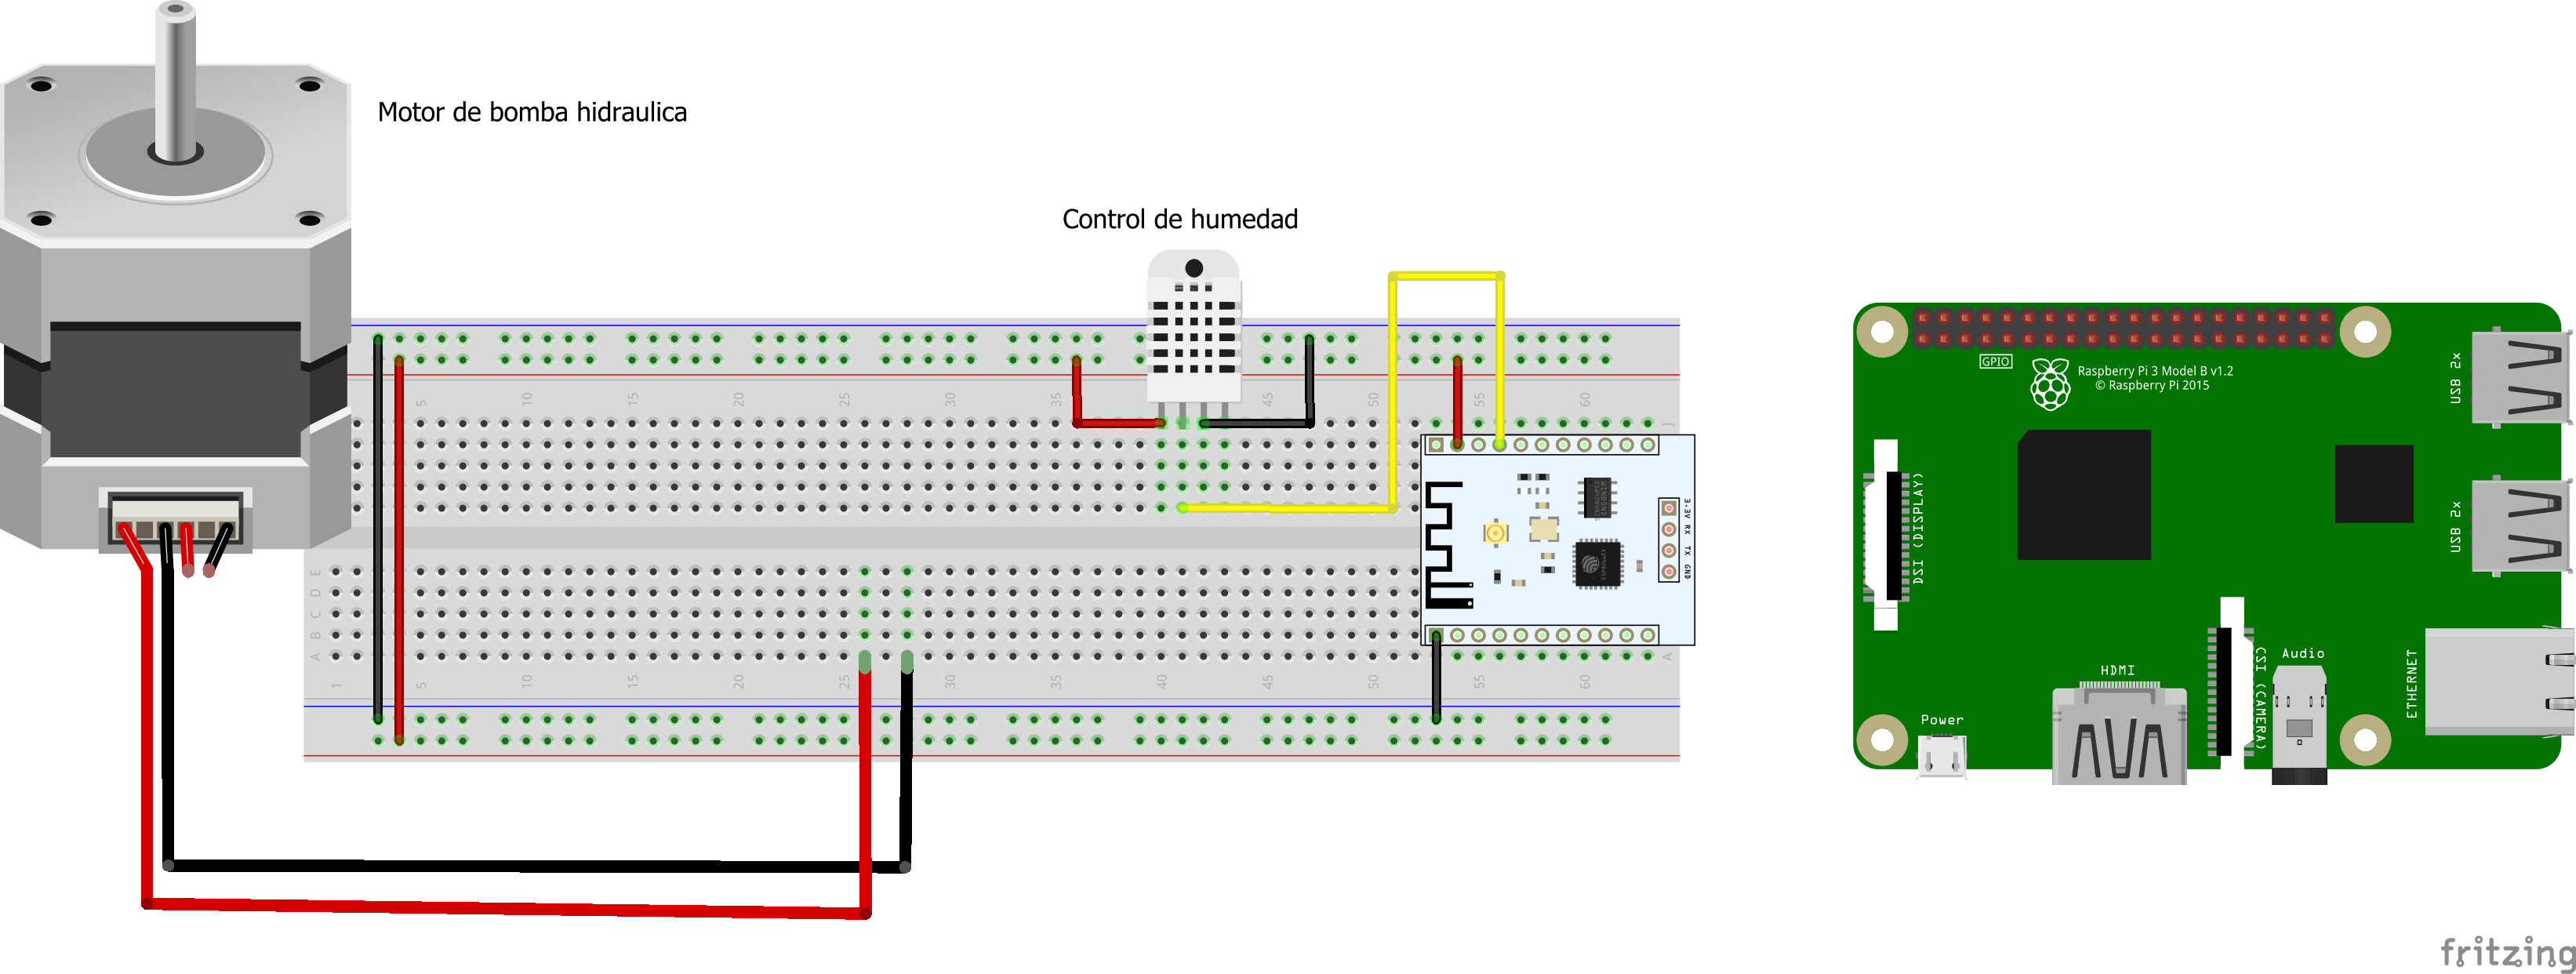
\includegraphics[scale=0.5]{./images/Conexion.png}
		\caption{Esquema básico de conexión Sensor-Sistema-Actuador}
		\label{Esquema_basico}
	\end{figure}		
	
	\subsubsection*{Sensores}

		\begin{itemize}
			\item Humedad.
			\item Fotovoltaico.
			\item Temperatura.
			\item Ph
		\end{itemize}

	\subsubsection*{Actuadores}

		\begin{itemize}
			\item Bomba de riego.
			\item Motores de paso.
			\item Servo Motores.
			\item Interruptor (Encendido y apagado del sistema).
			\item ...
		\end{itemize}			
	
	\subsubsection*{Controladores}
		
		\begin{itemize}
			\item RaspberriPi.
			\item ESP8266 | NodemCu.
		\end{itemize}			
	
	\subsubsection*{Información a tratar}
		
		\begin{itemize}
			\item \textbf{Sensores-ESP8266:} los datos del cultivo que controla.
			\item \textbf{ESP8266-Actuadores:} diferentes ordenes para mantener el cultivo que controla.
			\item \textbf{ESP8266-RasPi:} los datos recogidos de los sensores.
			\item \textbf{RasPi-ESP8266:} Intrucciones correspondientes a los datos externos recogidos (Lluvia, temperatura, sol,...). Información del usuario | Internet.
			
		\end{itemize}

\chapter{Funcionamiento}


\chapter{ToDos}

	\subsection*{Programación de los diferentes componentes [Ok]}
	
	\subsection*{Preparación del cableado, junto con la posible soldadura requerida [Ok]}
	
	\subsection*{Construcción del modelo de jardinería donde instalar todos los componentes[-]}
	
	\subsection*{Instalación de los diferentes componentes en la jardinera [-]}
	
	\subsection*{Instalación de la BBDD MongoDB [Ok]}
	
	\subsection*{Programación de la BBDD [Ok]}
	
	\subsection*{Instalación de la API Node-Red [-]}
	
	\subsection*{Programación de la API con Node-Red [-]}
	
	\subsection*{Probar el sistema y solucionar posibles fallos [-]}

\chapter{Ampliaciones}

	\subsection*{Motor de control de persiana}
	
\end{document}
